\mySection{Reportes}
En esta sección explicamos como generar los tres tipos de reportes que realiza el sistema: cantidad de consultas según prioridad, promedio de tiempos de espera según prioridad e historial de atenciones por paciente.

\mySubSection{Reporte de cantidad de consultas según prioridad}
Para acceder a la pantalla del reporte de cantidad de consultas según prioridad nos dirigimos hacia ``Reportes'' y luego a ``Prioridades'' (ver figura \ref{fig:menu_reporte_prioridades}).
\begin{figure}
\centerline{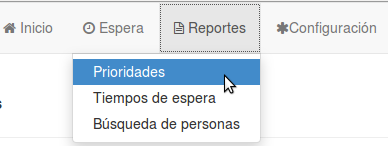
\includegraphics[width=0.7\textwidth]{menu_reporte_prioridades.png}}
\caption{Menú de reporte de prioridades}
\label{fig:menu_reporte_prioridades}
\end{figure}
Allí debemos ingresar la fecha inicial y la fecha final para delimitar las consultas a considerar dentro del reporte. Luego presionamos el botón ``Generar'' para obtener el reporte en pantalla (figura \ref{fig:reporte_prioridades}).
\begin{figure}
\centerline{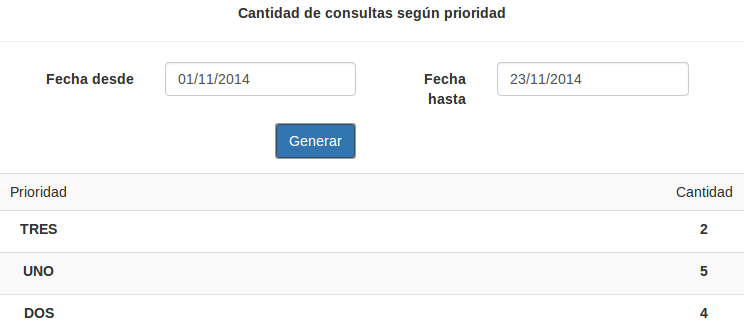
\includegraphics[width=1\textwidth]{reporte_prioridades.png}}
\caption{Reporte de cantidad de consultas según prioridad}
\label{fig:reporte_prioridades}
\end{figure}

\mySubSection{Reporte de promedio de tiempos de espera según prioridad}
Para acceder a la pantalla del reporte de promedio de tiempos de espera según prioridad nos dirigimos hacia ``Reportes'' y luego a ``Tiempos de espera'' (ver figura \ref{fig:menu_reporte_tiempos_espera}).
\begin{figure}
\centerline{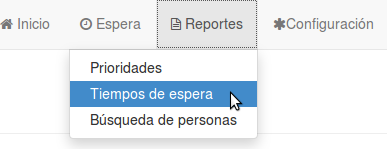
\includegraphics[width=0.7\textwidth]{menu_reporte_tiempos_espera.png}}
\caption{Menú de reporte de tiempos de espera}
\label{fig:menu_reporte_tiempos_espera}
\end{figure}
Allí, al igual que con el reporte de cantidad de consultas, debemos ingresar la fecha inicial y la fecha final para delimitar las atenciones a considerar dentro del reporte. Luego presionamos el botón ``Generar'' para obtener el reporte en pantalla (figura \ref{fig:reporte_tiempos_espera}).
\begin{figure}
\centerline{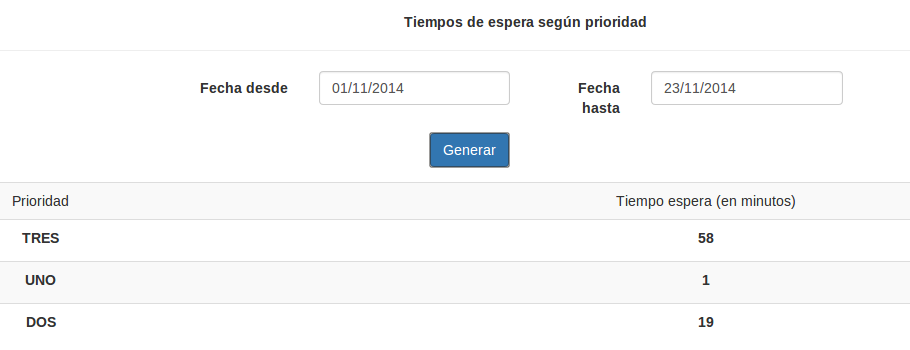
\includegraphics[width=1\textwidth]{reporte_tiempos_espera.png}}
\caption{Reporte de tiempos de espera según prioridad}
\label{fig:reporte_tiempos_espera}
\end{figure}

\mySubSection{Reporte de historial de atenciones por paciente}
Para acceder a la pantalla del reporte de historial de atenciones por paciente nos dirigimos hacia ``Reportes'' y luego a ``Búsqueda de personas'' (ver figura \ref{fig:menu_reporte_pacientes}).
\begin{figure}
\centerline{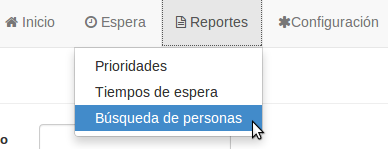
\includegraphics[width=0.7\textwidth]{menu_reporte_pacientes.png}}
\caption{Menú de reporte de historial de atenciones por paciente}
\label{fig:menu_reporte_pacientes}
\end{figure}
Allí podemos buscar el paciente que deseemos por DNI, apellido, fecha de nacimiento o nombre . Una vez encontrado el paciente presionamos el botón ``Detalle'' del listado (ver figura \ref{fig:listado_pacientes}) para ingresar en la pantalla del detalle de atenciones.
\begin{figure}
\centerline{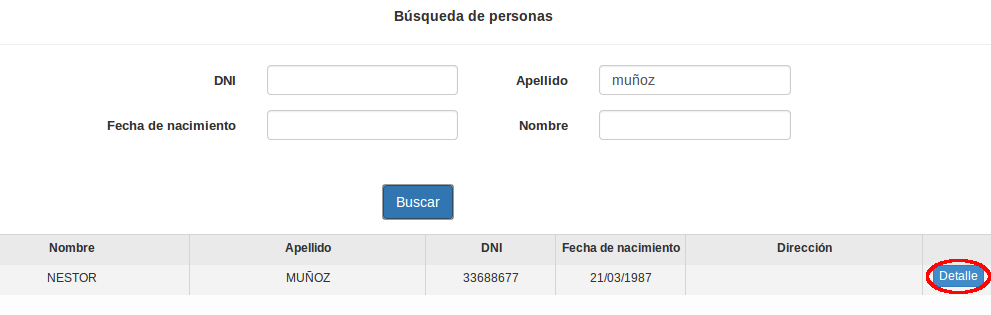
\includegraphics[width=1\textwidth]{listado_pacientes.png}}
\caption{Listado de pacientes}
\label{fig:listado_pacientes}
\end{figure}
Allí se nos muestran los datos personales del paciente más un listado con todas las atenciones que recibió (figura \ref{fig:historial_paciente}).
\begin{figure}
\centerline{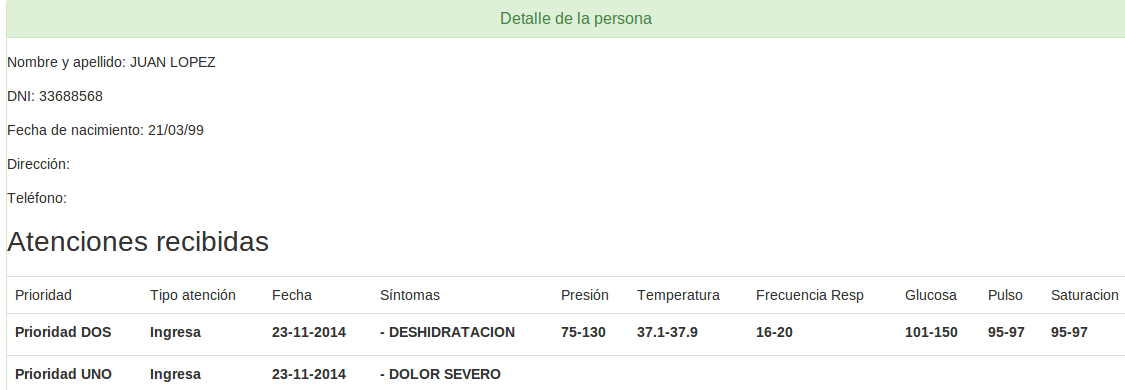
\includegraphics[width=1\textwidth]{historial_paciente.png}}
\caption{Historial de atenciones del paciente}
\label{fig:historial_paciente}
\end{figure}